\documentclass[12pt,fleqn]{article}\usepackage{../common}
\begin{document}
Ders 4

Duzlemin formulune donelim. 

\[ ax + by + cz = d \]

Bu formul $x,y,z$ noktalarinin bir duzlem uzerinde olma sartini tarif
ediyor. 

Su problemlere bakalim. Diyelim ki 

1) Orijinden, yani $(0,0,0)$ noktasindan gecen ve normal vektoru $\vec{N} = <1,5,10>$
olan bir duzlem yaratmak istiyoruz. Yani alttaki gibi bir sekil:

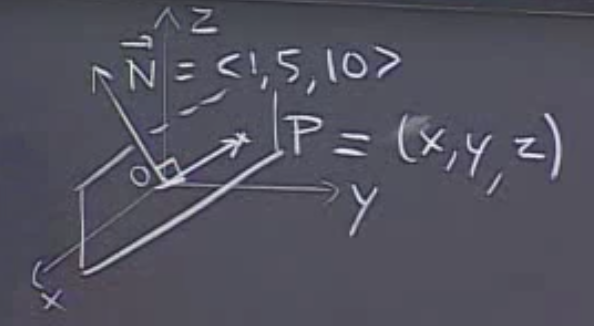
\includegraphics[height=4cm]{4_1.png}

Herhangi bir nokta $P = (x,y,z)$  ne zaman bu duzlem uzerindedir? Eger
orijinden $P$'ye giden vektor, duzlem normali ile doksan derece aci
olusturuyorsa. Yani $\vec{OP} \cdot \vec{N} = 0$ oldugu zaman $P$ noktasi
duzlem uzerindedir. 

Dikkat edelim, $x,y,z$ kordinatlarini, tek baslarina kullanir kullanmaz,
aslinda $\vec{OP}$'nin orijinden baslamasini sart kosmus oluyorum, cunku
$x,y,z$ kordinatlari sadece $(0,0,0)$ noktasina referansla anlamlilar. 

Her neyse, bu carpimi normal icin verdigimiz ornek sayilar icin yaparsak,
sonuc $x+5y+10 = 0$ olacaktir.

2) Simdi duzlem $P_0 = (2,1,-1)$ noktasindan gecsin (orijinden degil), ve
normal yine ayni olsun, $\vec{N} = <1,5,10>$. Bu durumu zihnimizde
canlandirmak icin yeni bir duzlemi hayal etmemiz lazim, ve $P$ noktasi bu
yeni duzlem uzerinde olacak.

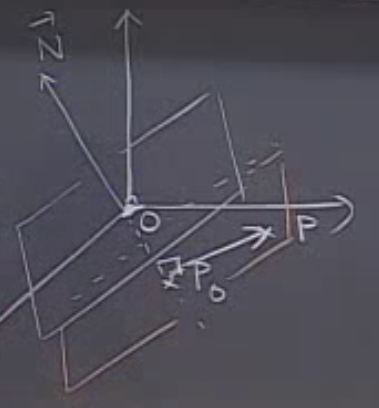
\includegraphics[height=4cm]{4_2.png}

$P$ ne zaman duzlem uzerinde? Eger 

\[ \vec{P_0P} \cdot \vec{N} = 0 \]

ise. O zaman 

\[ <x-2, y-1, z+1> \cdot <1,5,10> = 0 \]

\[ x+5y + 10z = -3 \]

$x,y,z$ uzerinde cikartma islemini niye yaptim? Cunku vektorun bir ucu hala
$x,y,z$ iceren $P$ noktasinda, diger ucu baslangic noktasi olan $P_0$'da.

1. problemdeki sonuctakiyle aradaki tek fark esitligin sagindaki -3
degeri. Bir benzerlik ise her iki durumda da $x,y,z$ katsayilarinin normal
vektorun degerlerine tekabul ediyor olmasi. Bu duzlemler hakkinda onemli
bir puf noktasi, eger orjinden geciyorlarsa esitligin sag tarafi sifir,
baska bir yerden geciyorlarsa, baska bir deger. Peki bu -3 degerini daha
hizli bir sekilde bulamaz miydik? Bulabilirdik. Cunku esitligin sol
tarafinin katsayilarini hizli bir sekilde bulabiliyoruz, orasi
tamam. Ayrica duzlemdeki bir noktanin kordinatlarini da biliyoruz, bu nokta
duzlemin icinden gecmesini sart kostugumuz $P_0$ noktasi. O zaman bu
kordinati $x,y,z$ terimlerini iceren formule koyarsak, esitligin sag
tarafini hemen hesaplariz. 

\[ x+5y + 10z = 1(2) + 5(1) + 10(-1) = 2 + 5 -10 = -3\]

Bu arada bir duzlemin tek bir formulu yoktur, sonsuz tane denklemi
vardir. Mesela her seyi 2 ile carpsaydim

\[ 2x+10y+20z = -6 \]

olurdu, ve bu formulde ayni denklemin formulu olurdu. Bunun coklugun sebebi
normal vektorlerin herhangi bir ``boyda'' olabilmesi, diklik icin yok
yeterli oldugu icin, farkli boylar ama degismeyen yon hala ayni duzlemi
tanimliyor. 

Duzlemi tanimlamak icin normal vektor en onemlisi. Bir onceki derste duzlem
uzerindeki noktalar, onlarin ortaya cikardigi iki vektor o vektorlerin capraz
carpimi uzerinden nasil normal vektor hesaplanabilecegini gormustuk.

Soru

Vektor $<1,2,-1>$ ve duzlem $x+y+3z = 5$ birbirine

\begin{enumerate}
   \item Paralel
   \item Dik
   \item Hicbiri
\end{enumerate}

Cevaplayin. 

Vektoru ve duzlemin normal vektorunu carptik. $<1,2,-1>\cdot<1,1,3> =
0$. 
Dogru cevap 1.

Simdi bir lineer denklem sistemini inceleyelim.

\[ x + z = 1  \]

\[ x + y = 2 \]

\[ x + 2y + 3z = 3 \]

Ilk iki denkleme bakalim. Bu denklem belli, ozel iki $x,z$ noktasindan
bahsediyor. Ikinci denklemi de gozonune alinca, ayni $x,z$ noktalarinin 
ikinci denklem icin de gecerli olmasi gerekir.

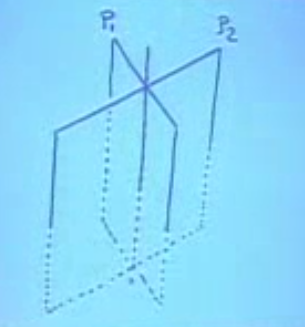
\includegraphics[height=3cm]{4_3.png}

Ilk iki denklemleri ayri duzlemler olarak dusunursek, cozum olacak $x,y,z$
iki duzlemin kesistigi yerdedir. Peki ucuncu denklem, yani ucuncu duzlem ne
yapar? 

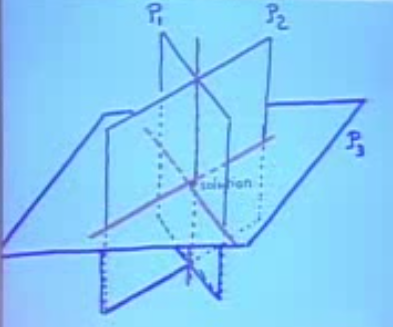
\includegraphics[height=3cm]{4_4.png}

O da iki duzlemin kesimindeki cizgiyi keser. Kesisimin kesimi bir
noktadir. O nokta da, ustteki lineer sistemin cozumu olan noktadir. 

Soru 

Eger 3 x 3 boyutlarindaki bir lineer sistemin cozumu bir nokta degilse,
nedir? 

\begin{enumerate} 
\item Cozum yoktur
\item Iki nokta (2 cozum)
\item Bir cizgi ($\infty$ tane cozum)
\item Bir tetrahedron
\item Bir duzlem
\item Bilmiyorum
\end{enumerate}

Diyelim ki ilk iki duzlemin kesismesi bir cizgi ortaya cikardi, ama bu
cizgi ucuncu duzlem ile paralel. O zaman cozum yok demektir. Fakat su da
dogru olabilir, belki bu cizgi ucuncu denklemin ``uzerindedir''. Bu durum
cebirsel olarak iki denklemin ortaya cikardigi bir denklemin ucuncu
denklemin kati olmasidir. Bu durumda ucuncu denklem bize hicbir yeni bilgi
saglamamistir. Bu durumda sonsuz tane cozum vardir, kesismeden ortaya
cikan cizgi uzerindeki ``her'' nokta bir cozumdur, ve sonsuza kadar uzayan
bir cizgi uzerinde sonsuz tane nokta vardir. 

O zaman dogru cevap 1, 3 ve 5.

5 niye dogru? Aynen iki denklemden ortaya cikan denklemin ucuncu denklemin
bir kati olmasi gibi, her uc denklem ayri ayri birbirinin kati olabilir. O
zaman bu denklemler aslinda ayni duzlemdirler. Cozum bu tek duzlemdir, ve
sonsuz tanedir. Yani size ayni denklemi uc kere vermisim demektir, bu pek
ilginc bir sistem sayilmaz, ama yine de bu bir lineer sistemdir. 

Soru

$x + y + z = ..$ gibi bir denklemin sagindaki sifir olmayan degerlerin
geometrik anlami nedir? Cevap: Daha once gordugumuz $x + y + z = 0$
orijinden gecer. Sag taraf sifir degilse, sifirdan gecen ayni duzleme
paralel ama ondan belli miktarda uzakta bir duzlemden bahsediyoruz
demektir. Ne kadar uzakta? Her zaman esitligin sagindaki buyukluk kadar
degil. O uzaklik icin hesabin ayrica yapilmasi lazim. Simdilik sadece
orijinden uzakta oldugunu bilelim. 

Simdi matrislere donelim. Onceki derste gordugumuz lineer cebir formulunu
hatirlayalim

\[ AX = B \]

\[ X = A^{-1}B \]

Buradaki problem, bir matrisin her zaman tersini alamayacagimiz gercegi. 

Hatirlarsak 

\[ A^{-1} = \frac{1}{det(A)}adj(A) \]

Bu hesapta eger determinant sifir cikarsa ustteki bolme islemini
yapamayiz. Yani bir onceki derste aslinda sunu soylememistik; bir matris
sadece determinanti sifir degilse tersine cevirilebilir. 

Geometrik olarak cozumun tek nokta oldugu durum, $A$'nin tersine
cevirilebilir oldugu durum. Kesisim cizgisinin ucuncu duzleme paralel
oldugu durum ise determinantin sifir, yani tersini cevirim yapilamadigi
durum. 

Homojen Durum

$AX = 0$ homojen durumdur, esitligin sagi sifirdir, yani uc denklem
orneginde tum denklemlerin sag tarafi sifirdir. 

Ornek

\[ x + z = 0 \]

\[ x + y = 0 \]

\[ x + 2y + 3z = 0 \]

Aslinda bu denklemin bariz ve hep mevcut bir cozumunu zaten
biliyoruz. $x,y,z$'nin hepsi sifir. Matematiksel terminolojide bu cozume
``basit cozum (trivial solution)'' denir. Geometrik anlami nedir? Her
denklemin sifira esit olmasi, onlarin temsil ettigi her duzlemin orijinden
gectigi anlamina gelir. Eh hepsi orijinden geciyorsa, hepsi orada
kesiyorlar da demektir. Basit cozum budur. 

Burada iki alt kalem / durum daha var. 

1) Eger $det(A) \ne 0$ o zaman $A$ tersine cevirilebilir, o zaman $X =
A^{-1} \ 0 = 0$. 
Baska hicbir cozum yoktur.

2) Eger $det(A) = 0$ o zaman $det(\vec{N_1},\vec{N_2},\vec{N_3}) = 0$, her
iki hesap ta sifir cunku normal vektorun ogeleri her denklemin $x,y,z$
katsayisi ayni zamanda, o katsayilari alip $A$ icine koyuyoruz, bu matrisin
determinantini hesaplamak bir baglamda normal vektorlerin determinantini
hesaplamakla esdeger oluyor. Devam edelim, uc formulu temsil eden uc
duzlemin normal vektorleri determinanti sifir, o zaman 
$\vec{N_1},\vec{N_2},\vec{N_3}$ ayni duzlemde (coplanar).

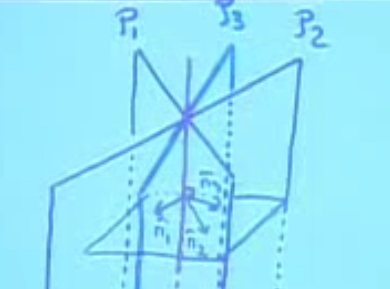
\includegraphics[height=4cm]{4_5.png}

$det(\vec{N_1},\vec{N_2},\vec{N_3})$ hesabinin paralelipipe hacmini hesapladigini hatirlayalim, ve 
bu hacim sifir ise vektorlerin olusturdugu hacim sifirdir, yani paralelipipe 
tamamen yassi demektir. O zaman vektorler ayni duzlemdedir. 

$\vec{N_1},\vec{N_2},\vec{N_3}$'nin ayni duzlemde ise, bu vektorlere ayni
anda dik olan bir cizgiyi dusunelim simdi. Iddia ediyorum ki o cizgi,
kesisme cizgisidir.

Niye? Cunku kesisme cizgim tum normal vektorlere ayni anda dik, yani o
normal vektorlerin temsil ettigi duzlemlerin hepsine ayni anda
paralel. Peki niye parallellik otesinde, o duzlemlerin ``uzerinde''? Cunku
cizgi orijinden geciyor, ve tum duzlemler de orijinden geciyor. Bunun
olabilmesi icin cizgim duzlemlerin uzerinde olmali.

O zaman elimde $\infty$ tane cozum vardir. 

Peki bu cozumleri nasil bulurum? $\vec{N_1} \times \vec{N_2}$ hesabi
$\vec{N_1},\vec{N_2}$'ye dik bir ucuncu vektor hesaplar, bunu biliyoruz, bu
vektor de $\vec{N_3}$'e ayni sekilde dik olmalidir cunku bu uc vektorun
ayni duzlemde oldugunu biliyoruz. Bu basit olmayan cozumdur.

Usttekiler homojen durum icindi. Simdi homojen olmayan, genel duruma duruma
bakalim.

Genel Durum (General Case)

Eger $det(A) \ne 0$ ise bir ozgun (unique) cozum vardir, $X = A^{-1}B$. 

Eger $det(A) = 0$ ise, ya hic cozum yoktur ya da sonsuz tane cozum
vardir. Tek bir cozum olmasi mumkun degildir. 

\end{document}
